%%% Partnership for Advanced Computing in Europe 
%%%   www.prace-ri.eu
%%%
%%% LaTeX example for a PRACE-RI whitepaper.
%%%
%%% (c) CSC - IT Center for Science Ltd.
%%%   author: Martti Louhivuori (martti.louhivuori@csc.fi)
%%%
%%% PRACE GENERIC LAYOUT; DO NOT CHANGE %%%
\documentclass{prace}
%%% END OF PRACE GENERIC LAYOUT %%%

% TITLE
\title{Example project report}

% AUTHORS
\author[1]{First Author}
\corresponding\author[1]{Second Author}
\author[1,2]{Third Author}

% AFFILIATIONS
\affiliation{Example University, Science Sq. 1, A City 01010, Random Country}
\affiliation{Institute for Advanced Examples, Factlane 11, Nosuchcity 12345,
Someland}

% PROJECT ID
\project{012345}

% CONTACT INFORMATION
\email{second.author@example.com}

%%% PRACE GENERIC LAYOUT; DO NOT CHANGE %%%
\begin{document}
\maketitle
%%% END OF PRACE GENERIC LAYOUT %%%

% ABSTRACT
\begin{abstract}
Lorem ipsum dolor sit amet, consectetuer adipiscing elit. Sed posuere interdum
sem. Quisque ligula eros ullamcorper quis, lacinia quis facilisis sed sapien.
Mauris varius diam vitae arcu. Sed arcu lectus auctor vitae, consectetuer et
venenatis eget velit. Sed augue orci, lacinia eu tincidunt et eleifend nec
lacus. Donec ultricies nisl ut felis, suspendisse potenti. Lorem ipsum ligula
ut hendrerit mollis, ipsum erat vehicula risus, eu suscipit sem libero nec
erat. Aliquam erat volutpat. Sed congue augue vitae neque. Nulla consectetuer
porttitor pede. Fusce purus morbi tortor magna condimentum vel, placerat id
blandit sit amet tortor.
\end{abstract}

% MAIN BODY
\section{Introduction}
This is an introductory section where some earlier
works\cite{scholes-DiscussFaradaySoc-70, mazurin-Phase-Separation-in-Glass-84} 
are cited like the one from Dimitriev and 
Kashchieva\cite{dimitriev-JMaterSci-75}. Also relevant 
background information is given as well as the goals of the project.

Lorem ipsum dolor sit amet, consectetuer adipiscing elit. Sed posuere interdum
sem. Quisque ligula eros ullamcorper quis, lacinia quis facilisis sed sapien.
Mauris varius diam vitae arcu. Sed arcu lectus auctor vitae, consectetuer et
venenatis eget velit. Sed augue orci, lacinia eu tincidunt et eleifend nec
lacus. Donec ultricies nisl ut felis, suspendisse potenti. Lorem ipsum ligula
ut hendrerit mollis, ipsum erat vehicula risus, eu suscipit sem libero nec
erat. Aliquam erat volutpat. Sed congue augue vitae neque. Nulla consectetuer
porttitor pede. Fusce purus morbi tortor magna condimentum vel, placerat id
blandit sit amet tortor.

Mauris sed libero. Suspendisse facilisis nulla in lacinia laoreet, lorem velit
accumsan velit vel mattis libero nisl et sem. Proin interdum maecenas massa
turpis sagittis in, interdum non lobortis vitae massa. Quisque purus lectus,
posuere eget imperdiet nec sodales id arcu. Vestibulum elit pede dictum eu,
viverra non tincidunt eu ligula.

Nam molestie nec tortor. Donec placerat leo sit amet velit. Vestibulum id
justo ut vitae massa. Proin in dolor mauris consequat aliquam. Donec ipsum,
vestibulum ullamcorper venenatis augue. Aliquam tempus nisi in auctor
vulputate, erat felis pellentesque augue nec, pellentesque lectus justo nec
erat. Aliquam et nisl. Quisque sit amet dolor in justo pretium condimentum.

Vivamus placerat lacus vel vehicula scelerisque, dui enim adipiscing lacus sit
amet sagittis, libero enim vitae mi. In neque magna posuere, euismod ac
tincidunt tempor est. Ut suscipit nisi eu purus. Proin ut pede mauris eget
ipsum. Integer vel quam nunc commodo consequat. Integer ac eros eu tellus
dignissim viverra. Maecenas erat aliquam erat volutpat. Ut venenatis ipsum
quis turpis. Integer cursus scelerisque lorem. Sed nec mauris id quam blandit
consequat. Cras nibh mi hendrerit vitae, dapibus et aliquam et magna. Nulla
vitae elit. Mauris consectetuer odio vitae augue.

\section{Methods}
Now we explain the methods used in the projects and go through the relevant
theoretical background\cite{eaton-Porous-Glass-Support-Material-75} with 
some equations like this
\begin{equation}
E = mc^2,
\label{eq: cliche}
\end{equation}
where we gave a definition for energy $E$ as a function of mass $m$ and speed
of light $c$. After this we can refer to the equation as Eq.~\ref{eq: cliche}.
Short in-line notation such as $a = b + c$ may also be used if needed, but 
should be avoided if possible.

And then if we want to use vectors or matrices we need to use bold typeface
for them, like this 
\begin{equation}
{\mathbf a} = {\mathbf b} \cdot \mathbf{c},
\label{eq: vectors}
\end{equation}
where we have simple vector dot product. More complex equations can also be
constructed using standard \LaTeX{} commands.

Lorem ipsum dolor sit amet, consectetuer adipiscing elit. Sed posuere interdum
sem. Quisque ligula eros ullamcorper quis, lacinia quis facilisis sed sapien.
Mauris varius diam vitae arcu. Sed arcu lectus auctor vitae, consectetuer et
venenatis eget velit. Sed augue orci, lacinia eu tincidunt et eleifend nec
lacus. Donec ultricies nisl ut felis, suspendisse potenti. Lorem ipsum ligula
ut hendrerit mollis, ipsum erat vehicula risus, eu suscipit sem libero nec
erat. Aliquam erat volutpat. Sed congue augue vitae neque. Nulla consectetuer
porttitor pede. Fusce purus morbi tortor magna condimentum vel, placerat id
blandit sit amet tortor.

\subsection{Some spiffy algorithm}
We also include a bullet-point list to outline the workflow of a
program:
\begin{itemize}
	\item initialise
	\item start main loop
	\begin{enumerate}
		\item calculate something
		\item write results to disk
		\item check whether we should terminate
	\end{enumerate}
	\item finalise
\end{itemize}
On top of that, we also have some schematic pictures to explain something
(Fig.~\ref{fig: example}).

\begin{figure}
	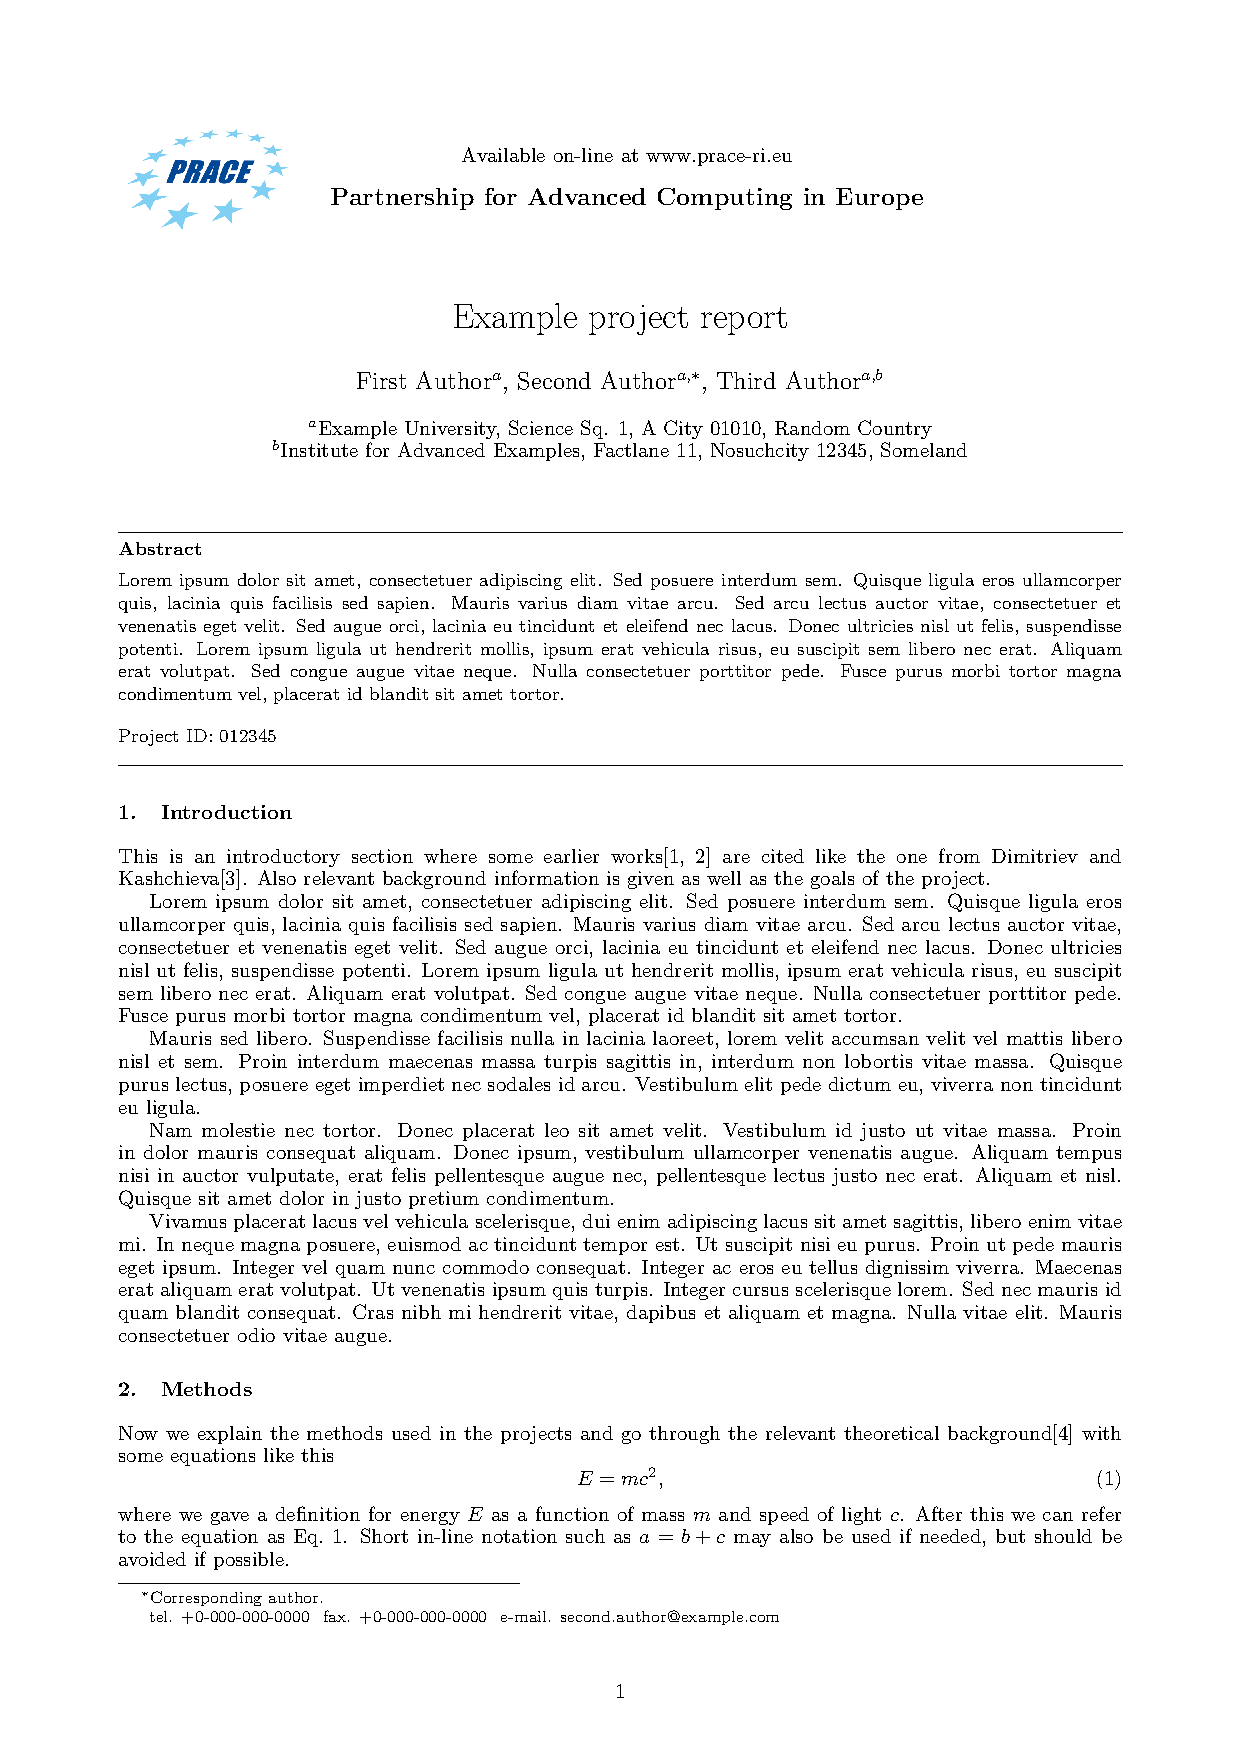
\includegraphics[width=0.4\textwidth]{example}\hfill{}
	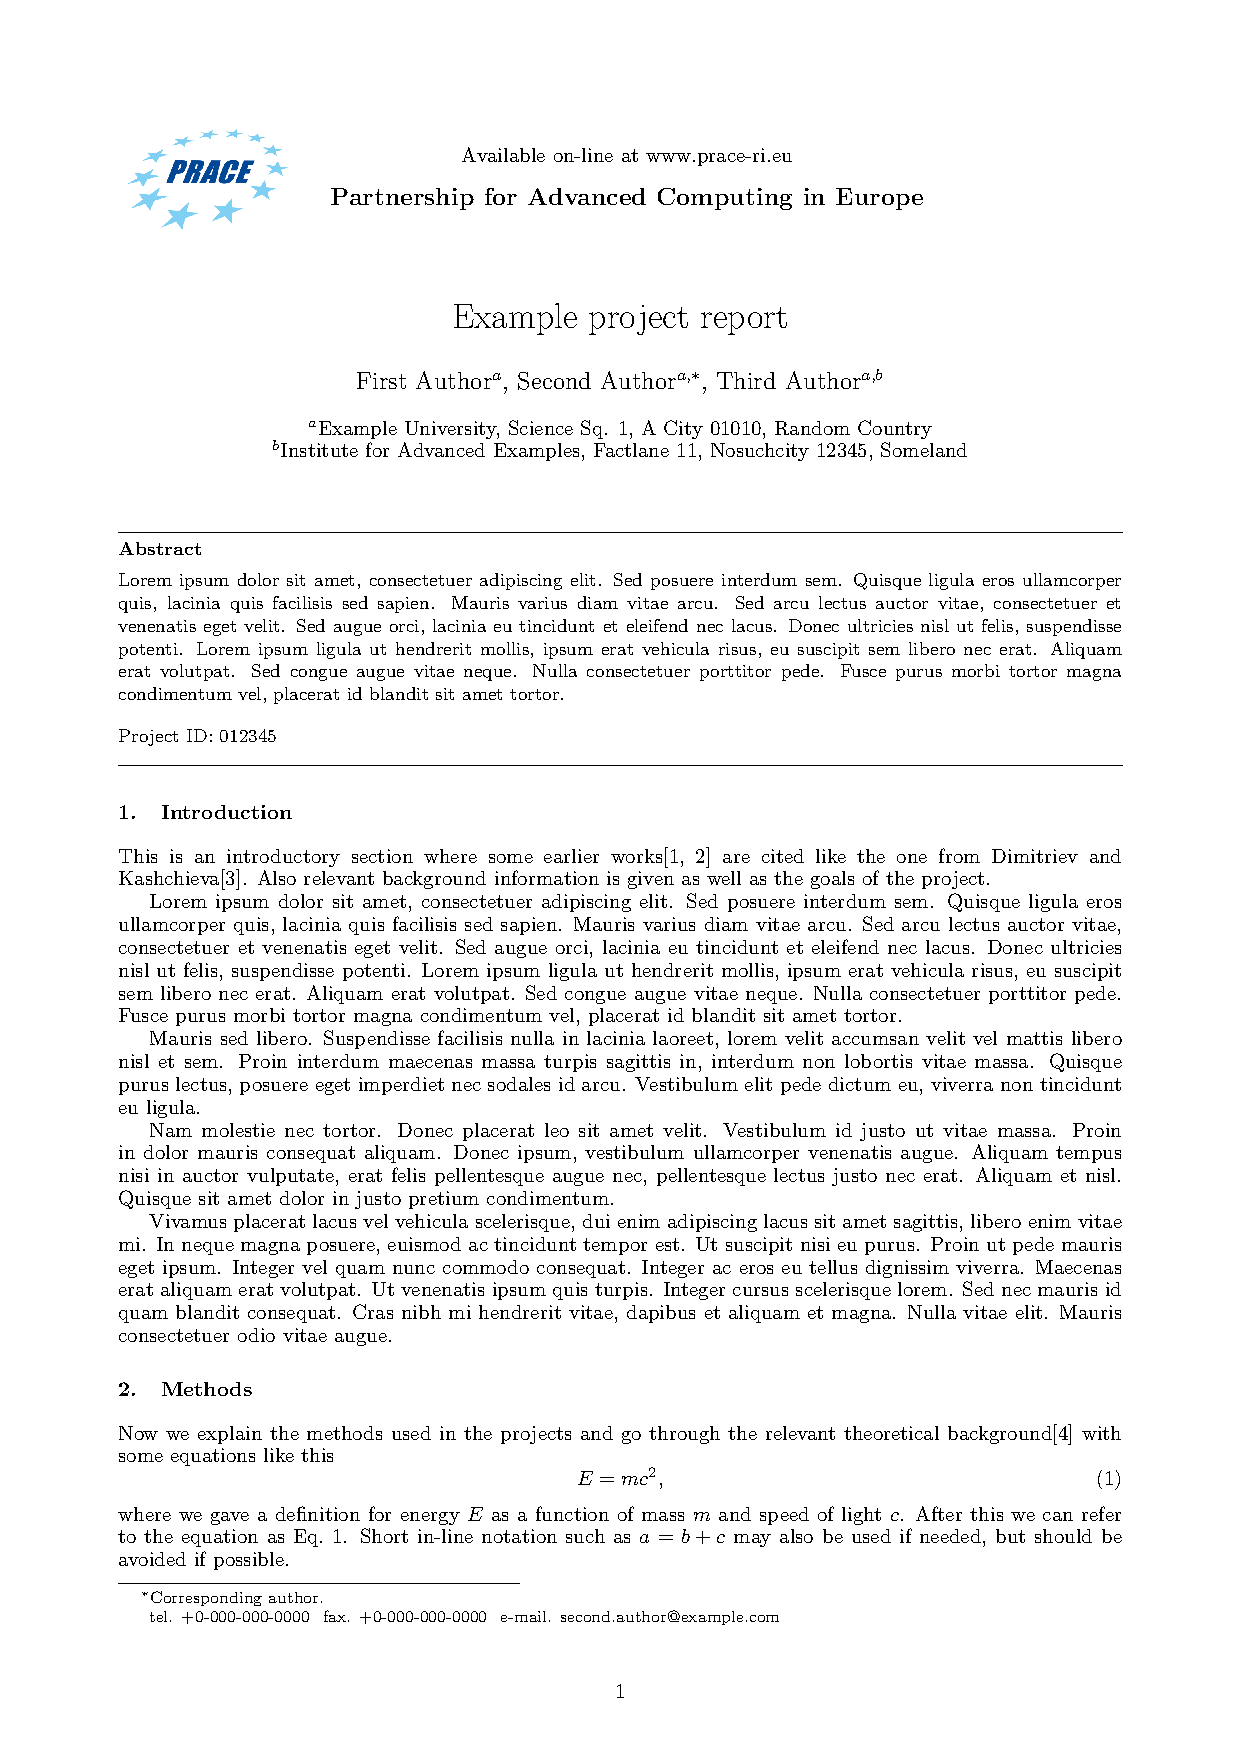
\includegraphics[width=0.4\textwidth]{example}\hfill{}
	\caption{(a) Example picture for the first time; (b) the same picture
	side-by-side with the first one.}
	\label{fig: example}
\end{figure}

Lorem ipsum dolor sit amet, consectetuer adipiscing elit. Sed posuere interdum
sem. Quisque ligula eros ullamcorper quis, lacinia quis facilisis sed sapien.
Mauris varius diam vitae arcu. Sed arcu lectus auctor vitae, consectetuer et
venenatis eget velit. Sed augue orci, lacinia eu tincidunt et eleifend nec
lacus. Donec ultricies nisl ut felis, suspendisse potenti. Lorem ipsum ligula
ut hendrerit mollis, ipsum erat vehicula risus, eu suscipit sem libero nec
erat. Aliquam erat volutpat. Sed congue augue vitae neque. Nulla consectetuer
porttitor pede. Fusce purus morbi tortor magna condimentum vel, placerat id
blandit sit amet tortor.

Mauris sed libero. Suspendisse facilisis nulla in lacinia laoreet, lorem velit
accumsan velit vel mattis libero nisl et sem. Proin interdum maecenas massa
turpis sagittis in, interdum non lobortis vitae massa. Quisque purus lectus,
posuere eget imperdiet nec sodales id arcu. Vestibulum elit pede dictum eu,
viverra non tincidunt eu ligula.

Nam molestie nec tortor. Donec placerat leo sit amet velit. Vestibulum id
justo ut vitae massa. Proin in dolor mauris consequat aliquam. Donec ipsum,
vestibulum ullamcorper venenatis augue. Aliquam tempus nisi in auctor
vulputate, erat felis pellentesque augue nec, pellentesque lectus justo nec
erat. Aliquam et nisl. Quisque sit amet dolor in justo pretium condimentum.

Vivamus placerat lacus vel vehicula scelerisque, dui enim adipiscing lacus sit
amet sagittis, libero enim vitae mi. In neque magna posuere, euismod ac
tincidunt tempor est. Ut suscipit nisi eu purus. Proin ut pede mauris eget
ipsum. Integer vel quam nunc commodo consequat. Integer ac eros eu tellus
dignissim viverra. Maecenas erat aliquam erat volutpat. Ut venenatis ipsum
quis turpis. Integer cursus scelerisque lorem. Sed nec mauris id quam blandit
consequat. Cras nibh mi hendrerit vitae, dapibus et aliquam et magna. Nulla
vitae elit. Mauris consectetuer odio vitae augue.

\section{Results}
Here we present the results of the projects with some tables and figures.
Subsections could also be used to organise the content into smaller parts. For
this example we don't care to do so, but we do include a nice summary of the
main results in Table~\ref{tab: results}.

\begin{table}
	\caption{Example table of project results.}
	\label{tab: results}
	\begin{tabular}{llll}
		\toprule
		\multicolumn{2}{c}{sample} & {} \\
		\cmidrule(lr){1-2}
		entry & set & {} time (s) & temperature (K) \\
		\midrule
		example 1 & a & 1 & 2 \\
		{} & z & 3 & 4 \\
		example 2 & i & 5 & 6 \\
		\bottomrule
	\end{tabular}
\end{table}

Lorem ipsum dolor sit amet, consectetuer adipiscing elit. Sed posuere interdum
sem. Quisque ligula eros ullamcorper quis, lacinia quis facilisis sed sapien.
Mauris varius diam vitae arcu. Sed arcu lectus auctor vitae, consectetuer et
venenatis eget velit. Sed augue orci, lacinia eu tincidunt et eleifend nec
lacus. Donec ultricies nisl ut felis, suspendisse potenti. Lorem ipsum ligula
ut hendrerit mollis, ipsum erat vehicula risus, eu suscipit sem libero nec
erat. Aliquam erat volutpat. Sed congue augue vitae neque. Nulla consectetuer
porttitor pede. Fusce purus morbi tortor magna condimentum vel, placerat id
blandit sit amet tortor.

Mauris sed libero. Suspendisse facilisis nulla in lacinia laoreet, lorem velit
accumsan velit vel mattis libero nisl et sem. Proin interdum maecenas massa
turpis sagittis in, interdum non lobortis vitae massa. Quisque purus lectus,
posuere eget imperdiet nec sodales id arcu. Vestibulum elit pede dictum eu,
viverra non tincidunt eu ligula.

\section{Summary}
Nam molestie nec tortor. Donec placerat leo sit amet velit. Vestibulum id
justo ut vitae massa. Proin in dolor mauris consequat aliquam. Donec ipsum,
vestibulum ullamcorper venenatis augue. Aliquam tempus nisi in auctor
vulputate, erat felis pellentesque augue nec, pellentesque lectus justo nec
erat. Aliquam et nisl. Quisque sit amet dolor in justo pretium condimentum.

Vivamus placerat lacus vel vehicula scelerisque, dui enim adipiscing lacus sit
amet sagittis, libero enim vitae mi. In neque magna posuere, euismod ac
tincidunt tempor est. Ut suscipit nisi eu purus. Proin ut pede mauris eget
ipsum. Integer vel quam nunc commodo consequat. Integer ac eros eu tellus
dignissim viverra. Maecenas erat aliquam erat volutpat. Ut venenatis ipsum
quis turpis. Integer cursus scelerisque lorem. Sed nec mauris id quam blandit
consequat. Cras nibh mi hendrerit vitae, dapibus et aliquam et magna. Nulla
vitae elit. Mauris consectetuer odio vitae augue.

Cras lobortis sem ultrices leo. Donec magna fusce ac ante. Nullam est nisi
blandit eget, suscipit vitae posuere quis ante. Quisque vitae tortor tellus
feugiat adipiscing. Morbi ac elit et diam bibendum bibendum. Suspendisse id
diam, donec adipiscing vulputate metus. Cras pellentesque vestibulum sem.
Maecenas ut elit quis nisl vestibulum bibendum. Aenean eu erat quis turpis
consequat vehicula. Morbi lacus velit, tristique ut iaculis volutpat in velit.
Duis nec mauris et velit mollis aliquam, nullam posuere. Mauris at turpis sit
amet dui imperdiet lobortis, proin eu felis.

\section*{Acknowledgements}
This work was financially supported by the PRACE project funded in part
by the EUs 7th Framework Programme (FP7/2007-2013) under grant agreement
no. RI-283493. The work was achieved using the PRACE Research Infrastructure
resources at the CURIE (GENCI), the FERMI (CINECA), and the SuperMUC (LRZ)
supercomputers.

% REFERENCE LIST
\begin{thebibliography}{99}

\bibitem{scholes-DiscussFaradaySoc-70}
S. Scholes, Discuss. Faraday Soc. No. 50 (1970) 222.

\bibitem{mazurin-Phase-Separation-in-Glass-84}
O.V. Mazurin and E.A. Porai-Koshits (eds.), 
Phase Separation in Glass, North-Holland, Amsterdam, 1984.

\bibitem{dimitriev-JMaterSci-75}
Y. Dimitriev and E. Kashchieva, J.Mater. Sci. 10 (1975) 1419.

\bibitem{eaton-Porous-Glass-Support-Material-75}
D.L. Eaton, Porous Glass Support Material, US Patent No. 3 904 422 (1975).

\end{thebibliography}

%%% PRACE GENERIC LAYOUT; DO NOT CHANGE %%%
\end{document}
%%% END OF PRACE GENERIC LAYOUT %%%
